% !TEX root = ../Tesis_NataliaOpazo.tex

La consideraci\'on del papel relativo que ha jugado la variabilidad natural y/o los factores
antr\'opicos en la modificaci\'on de ambientes a escala local y global es de vital importancia a la
hora de abordar una de las grandes problem\'aticas ambientales actuales, el cambio clim\'atico.
La preocupaci\'on social en torno al incremento de gases invernadero en la atm\'osfera y su
repercusi\'on en el clima es cada d\'ia mayor. \\
El clima actual es el resultado de la evoluci\'on de las condiciones ambientales del planeta
desde su formaci\'on. Las condiciones clim\'aticas actuales s\'olo se pueden entender si se
entiende la historia clim\'atica de la Tierra. 

El clima ha ido oscilando
de forma peri\'odica entre \'epocas glaciales y \'epocas m\'as c\'alidas
llamadas interglaciares, respondiendo a procesos de la tectónica, a cambios en parámetros orbitales y a retroalimentaciones internas de la tierra \citep{sleep2001carbon,barker2009interhemispheric,toggweiler2006midlatitude}. Si bien durante el Cuaternario el efecto directo de los parámetros orbitales pudo explicar gran parte de las variaciones hacia finales del Pleistoceno \citep{denton2010last}, no es suficiente para explicar la amplitud y la cantidad de transiciones climáticas registradas, razón por la cual retroalimentaciones internos estarían jugando un rol importante en los cambios energéticos.

\cite{luthi2008high}, mostró que existe una notable correlaci\'on entre el contenido de $CO_2$ atmosférico y la temperatura de los \'ultimos
800 miles de a\~nos. No obstante, aún permanecen esquivos los mecanismos responsables de las fluctuaciones
atmosf\'ericas de $pCO_2$, donde los registros muestran que han variado entre los rangos de valores de 80 a 100 p.p.m.v, con mínimos valores durante periodos glaciares y máximos durante interglaciares \citep{sigman2000glacial}.

Investigaciones en varios reservorios que intercambian $CO_2$ con la atm\'osfera han mostrado evidencias de la gran capacidad del océano para capturar y almacenar CO$_2$ atmosférico mediante su actividad biológica \citep{martinez2014iron} y características físicas, lo que los ha llevado a concluir que es el océano el que maneja los cambios en el CO$_2$ atmosférico y, por lo tanto, que tiene un rol importante en las variaciones climáticas. 


\section{Ciclo del carbono}

Dentro del ciclo del carbono, existe un ciclo que actúa a escalas temporales que van desde los $100000$ hasta 1 Millón de años \citep{sleep2001carbon}. Este proceso está particularmente relacionado con la erosión de silicatos en pos de la formación de carbonatos, la cual se da en condiciones de bajas temperaturas y viceversa. 

\begin{equation} \label{eq:marco1.1}
CO_{2} + CaSiO_{3 s\acute{o}lido} \rightleftharpoons SiO_{2} + CaCO_{3}
\end{equation}

Donde la eventual meteorización de rocas produce una disolución del carbonato y liberación de (Ca$^{2+}$) (ver ecuación \ref{eq:marco1.2.1}) las que mediante la escorrentía u otros procesos pueden llegar al océano, donde la biolog\'ia presente intervendr\'a para que el (Ca$^{2+}$) reaccione y forme el CaCO${_3}$. Posteriormente, si los carbonatos eventualmente alcanzan el fondo marino, dada la mayor disponibilidad de CO$_2$ (entorno m\'as \'acido, ver ecuaci\'on \ref{eq:marco1.2.1}), la reacci\'on \ref{eq:marco1.1} se invierte, produci\'endose una transformaci\'on de gran parte de los carbonatos que se encuentran profundamente en la corteza, de la forma:

\begin{equation} \label{eq:marco1.2.1}
H_{2}O + CO_{2} + CaCO_{3} \rightleftharpoons Ca^{2+} + 2HCO_{3}^{-}
\end{equation}

 No obstante, una minúscula parte logrará ingresar en el manto por procesos de subducción de la corteza marina \citep{sleep2001carbon,raymo1992tectonic}. 
 Sin embargo, este proceso también tiene su inverso, dado que es mediante la vulcanización o formación de nueva corteza marina o terrestre, que este CO$_2$ puede retornar a la atmósfera (ver figura \ref{fig:marc0.1}). \\

 \begin{figure}[H]
\centering
 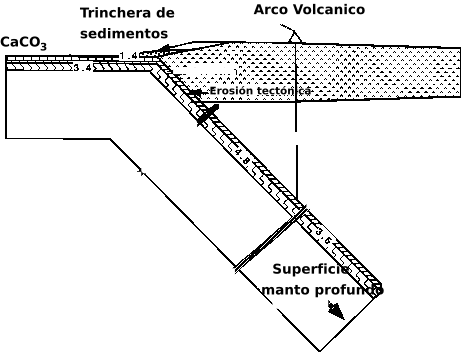
\includegraphics[width=0.6\textwidth]{tectonica.png}
 \caption[Ciclo del carbonato]{Representación del carbonato en la plataforma marina. Imagen modificada de \citep{sleep2001carbon}.}
  \label{fig:marc0.1}
\end{figure}


\subsection{Bomba biológica}

Si bien existe un ciclo del carbono que opera lentamente, también veremos a continuación un ciclo de carbono que funciona de forma paralela relacionado con los procesos biológicos, lo que hace que tenga escalas temporales más cortas y que esté directamente relacionado con la variabilidad climática \citep{sigman2003biological}. Así veremos la biogeoquímica que involucra la llamada \textit{bomba biológica}, en términos de los balances de carbono orgánico en el océano, sin considerar los ciclos y balances inorg\'anicos involucrados. \newpage

\begin{figure}[H]
\centering
 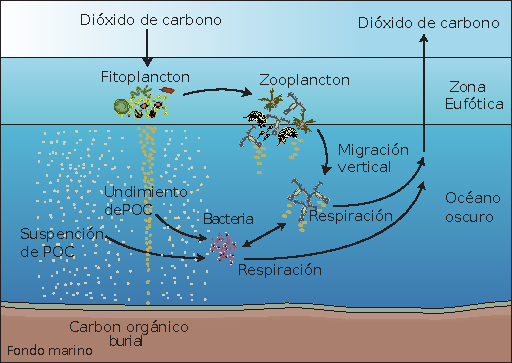
\includegraphics[width=0.9\textwidth]{pump.pdf}
 \caption[Modelo simple efecto bomba biológica]{Modelo simple efecto bomba biológica. La fijación fotosintética del carbono en la materia orgánica producida por el fitoplancton en la zona iluminada del océano (Carbono orgánico particulado, POC por sus siglas en inglés). Junto con la asimilación de macro y micro-nutrientes tales como, el nitrógeno, fosfato, hierro (principales limitantes) entre otros. Impulsa procesos de liberación de materia orgánica en esta capa, que son en su mayoría respirados y remineralizados. De la porción que logra escapar y se exporta al océano interior oscuro (zona afótica), una parte pequeña seguirá su camino hasta llegar a los sedimentos del fondo oceánico, mientras que la mayoría se remineralizará y oxidará a sus formas inorgánicas, gran parte de estas formas inorgánicas serán trasladadas de regreso a la zona eufótica producto de la circulación y mezcla, donde abastecerá de nutrientes a un nuevo crecimiento. Modificado de \citep{herndl2013microbial}.}
  \label{fig:bio1}
\end{figure} 

Producto de una diferencia en la presi\'on parcial del CO$_2$ gaseoso en la interfase oc\'eano-atm\'osfera y considerando que la presi\'on parcial de $CO_2$ tiende a estar en equilibrio, su aumento en la atm\'osfera fuerza un flujo hacia el oc\'eano. Cuando este gas entra en el océano, dentro de la gran variedad de ecosistemas que lo habitan, existen unos organismos llamados \textit{autótrofos}, que son aquellos que convierten este CO$_2$ en carbono orgánico. Esta conversión ocurre durante la \textit{fotosíntesis}, donde se utiliza como fuente de energía la luz solar, que mediante pigmentos, principalmente la clorofila, se transforma esta energía solar a energía química. La biomasa que realiza este proceso esta conformada mayormente por plancton en su forma bacterial (bacterioplancton), vegetal (fitoplancton) o animal (zooplancton) \citep{jeandelmarine}. Así el $CO_2$ entra en todos los constituyentes moleculares de estos organismo, en la forma

\begin{equation} \label{eq:marco1.2}
CO_{2} + H_{2}O + \textrm{energía solar} \rightleftharpoons CH_{2}O + O_{2}
\end{equation}

la fotosíntesis ocurre en la zona iluminada del océano (zona fótica), donde la profundidad de ésta capa de agua puede variar desde unos pocos metros (en zonas con alta turbulencia), hasta aproximadamente $150$ metros en aguas claras y con poca productividad. Además del carbono se requieren de otros macronutrientes para llevar a cabo la \textit{fotosíntesis}, tales como el nitrógeno (nitrato, NO$^{-}_{3}$), el fósforo (fosfato, PO$^{3-}_{4}$) y sulfato. Así la formación de la materia orgánica se puede ver

\begin{equation} \label{eq:marco1.3}
\begin{split}
106CO_{2} + 16HNO_{3} + 1H_{3}PO_{4} +122H_{2}O+ \textrm{energía solar} \rightleftharpoons \\
(CH_{2}O)_{106}(NH_{3})_{16}(H_{3}PO_{4})  + 138O_{2}
\end{split}
\end{equation}

Se aprecia la fijación de nitrógeno (NO$^{-}_{3}$) y CO$_2$ mediante la asimilación de ácido nítrico (HNO$_{3}$) para dar forma a los hidratos de carbono y aminoácidos (amonio), con la consecuente incorporación de fosfato para sintetizar las moléculas orgánicas. \\

La formación y productividad del fitoplancton estarán entonces relacionadas con la presencia u ausencia de carbono, nitrógeno y fosfato, en una proporción constante, que según \cite{redfield1934proportions} es C:N:P = 106/16/1. Sin embargo, a pesar de que el nitrógeno molecular (N$_2$) es muy abundante, existen pocos organismo que lo pueden absorber directamente, debido a que necesitan alta energía para lograr romper su triple enlace covalente, razón por la cual el balance entre la asimilación de N$_2$ a nitrógeno orgánico (fijación de nitrógeno) junto con la conversión de nitrato (desnitrificación) a N$_2$, son de vital importancia para el nitrógeno y para el inventario de nitrógeno biodisponible en la productividad marina. Por otro lado el PO$_{4}^{3-}$, es principalmente suministrado al océano por ríos, pero este aporte tiene mayor impacto en zonas costeras, en el océano abierto el suministro a la zona superficial deriva de procesos de surgencia o volcamiento oceánico, por ende, el PO$_{4}^{3-}$ utilizado por los organismos proviene mayormente de procesos de reciclaje. Así, muchas zonas del océano superficial tienen escasa o mínima concentración de NO$_{3}^{-}$ y PO$_{4}^{3-}$, que son consumidos completamente por el fitoplancton, lo que los hace los llamados elementos limitantes, es decir, que limitan el desarrollo del fitoplancton \citep{archer2000caused}. Entre estos también destaca el ácido silicio (Si(OH)$_4$) utilizado para construir los esqueletos de muchas especies de plancton, pero que es particularmente consumido por las diatomeas, un importante especie de fitoplancton responsable de gran parte de la producción de exportación de la tierra. Esta especie es menos propensa al consumo de fitoplancton por zooplancton (pastoreo), requiere de sílice en la forma de (Si(OH)$_4$) para el crecimiento y producción de sus frústulas (sílice biogénica, bSiO$_2$), lo cual luego será exportado en forma de sílice opalina \citep{treguer2000global,arellano2011high}. Además micronutrientes como el hierro (Fe) que será responsable de limitar la fijación de nitrógeno, dada su acción en la formación de la \textit{nitrogenasa} enzima del fitoplancton sintetizadora del nitrógeno molecular (N$_2$), una de las entradas más importantes de nitrógeno en regiones oligotróficas del océano \citep{mahaffey2005conundrum,gruber2008marine}. 

Por otro lado, el CO$_2$ que es asimilado por el fitoplancton está en su estado de carbono inorgánico disuelto (DIC), que se deriva de la reacción 

\begin{equation} \label{eq:marco1}
CO_{2 (g)} + H_{2}O\rightleftharpoons H_{2}CO_{3} \rightleftharpoons H^{+} + HCO_{3}^{-1} \rightleftharpoons 2H^{+} + CO_{3}^{-2} 
\end{equation}

El proceso qu\'imico que esta detr\'as de este mecanismo es el siguiente: el $CO_2$ cuando ingresa al agua de mar, se disuelve en el agua (producto de la temperatura y salinidad), reacciona con ella para formar \'acido carb\'onico $H_{2}CO_{3}$, pero este en general es inestable por ende tiende a liberar protones formando el i\'on carbonato de hidr\'ogeno $HCO_{3}^{-1}$ (bicarbonato) y el i\'on carbonato $CO_{3}^{-2}$ (carbonato), los que conjuntamente aumentan considerablemente la concentraci\'on de DIC en el agua\citep{Turekiangeochemistry}. El $CO_2$ como gas disuelto est\'a en muy peque\~nas cantidades, no alcanza el 2\% de la $\sum CO_2$ (suma de todas las concentraciones de las especies químicas del dióxido de carbono disuelto). La especie qu\'imica m\'as abundante en el oc\'eano es el bicarbonato, aproximadamente el 90\% del $CO_2$ que entra en el mar se encuentra en forma de i\'on bicarbonato y un $\sim$8\% en forma de i\'on carbonato. El $HCO_{3}^{-1}$ es m\'as consumido por procesos de fotos\'intesis que el CO$_2$ disuelto.

La materia orgánica que es producida por el fitoplancton, así como agregados de celular muertas, cuerpos de zooplancton o heces son consumida por bacterias heterótrofas y zooplancton.  Es rápida y generalizadamente remineralizada en la zona superficial, parte sin embargo, deja la zona eufótica para precipitarse hacia el océano profundo. No obstante, en esta lluvia de materia orgánica, esta materia es consumida por bacterias y animales, lo que hace que la materia se oxide y vuelva a sus componentes minerales, por esta razón, la concentración de nutrientes inorgánicos aumenta con la profundidad, a este proceso se le suele denominar ``respiración o remineralización'', alcanzando un máximo en torno a los 1000 metros de profundidad. 
Este proceso de consumo y liberación de nutrientes se puede ver como

\begin{equation} \label{eq:marco1.4}
\begin{split}
(CH_{2}O)_{106}(NH_{3})_{16}(H_{3}PO_{4})  + 138O_{2} \rightleftharpoons \\
106CO_{2} + 16HNO_{3} + 1H_{3}PO_{4} +122H_{2}O+ \textrm{energía química} 
\end{split}
\end{equation}

El nitrógeno, fosfato, DIC y hierro, siguen estas rutas como se puede apreciar en la figura \ref{fig:bio1}. Así, la remineralización ejerce procesos inversos en el océanos profundo. Por un lado, en ausencia de fotosíntesis, la concentración de nutrientes en su estado inorgánico aumentará en profundidad. Mientras que el carbono orgánico disuelto (DOC), o en su estados más pequeño particulado (POC) serán más altos en superficie y comenzarán a disminuir en profundidad. 

Finalmente, sólo el $1\%$  \citep{gruber2008marine} de la materia orgánica que logra alcanzar el lecho marino se almacena finalmente en los sedimentos del fondo oceánico (puede ser mayor en zonas costeras), y se reintegra al ciclo geológico del carbono. \newpage

\subsection{Volcamiento oceánico}

\begin{figure}[H]
\centering
 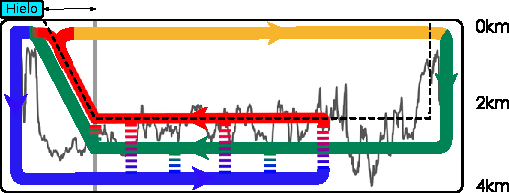
\includegraphics[width=0.7\textwidth]{ferrari2014antarctic.pdf}
 \caption[Circulación de volcamiento]{Circulación de volcamiento. La linea azul es la \textit{Agua Profunda de la Antártica}, la barra verde es la \textit{Agua profunda del Atlántico Norte}, la barra roja es el \textit{Agua Profunda de la India y del Pacífico} y la línea amarilla es la \textit{Agua Intermedia Antártica}. Imagen obtenida y modifica de \cite{ferrari2014antarctic}.}
  \label{fig:circ}
\end{figure}

La concentración de componentes inorgánicos almacenados en el océano profundo entre ellos el DIC, podrá volver a las aguas superficiales del océano por transporte de corrientes oceánicas o por procesos de surgencia. Este proceso de exposición de aguas profundas se da cada aproximadamente 1000 años \citep{sigman2000glacial}, donde el CO$_2$ ocasionalmente podr\'a ser liberada a la atm\'osfera, y los otros componentes reutilizados por la biolog\'ia. En este sentido, la \textit{circulación termohalina} (CTH) genera un transporte meridional de nutrientes y de DIC, que en procesos de ventilación oceánica, son importantes fuentes de carbono hacia la atmósfera \citep{toggweiler2006midlatitude}.  

La CTH es un gran transportado oceánico. La que ``comienza'' en la formación de aguas profundas en la zona del Atlántico norte (NADW) y en la Ant\'artica (AABW). Donde la NADW ser\'a desplazada en profundidad hacia el sur donde converger\'a con las aguas profundas y densas AABW, con las que producto de procesos de mezcla formará las aguas de la corriente Circumpolar profunda (CDW), las que llegará a superficie en la zona del Círculo Polar Antártico (ACC). Esta surgencia en superficie, estará siendo forzada por procesos de divergencia de aguas generado por los vientos del oeste. De esta manera, por transporte de Ekman la componente norte del afloramiento de aguas será trasladada a través de las termoclina de las distintas cuencas oceánicas (océano Índico, Pacífico y Atlántico) antes de retornar a la zona de hundimiento del océano Atlántico Norte (ver figura \ref{fig:circ}). Mientras, la componente sur del afloramiento de la CDW por diferencias de densidad, se hunde devuelta al océano profundo. 

A lo largo de este cinturón de corrientes se ve expuesta la actividad biológica. En zonas de surgencia o afloramiento oceánico se llevarán a superficie grandes contenidos de nutrientes inorgánicos, como el DIC, producido como vimos por procesos de remineralización y respiración en profundidad. Mientras, que en zonas de hundimiento o ``formación'' de aguas profundas, se verán secuestrados grandes contenidos de DIC producto de la utilización de nutrientes en superficie. 

 La CTH, no tan sólo es responsable del transporte de nutrientes por parte corrientes profundas y superficiales, si no además, es un gran transportador de calor en el océano. 

\subsection{Suministro de nutrientes}

En la producci\'on de materia org\'anica existen elementos que a menudo limitan la fotos\'intesis. Es usual hacer la distinci\'on entre macronutrientes (N y P) y micronutrientes 
(elementos traza) de acuerdo a su concentraci\'on relativa en los organismos. La concentraci\'on media de macronutrientes es del orden de los $mmol\ m^{-3}$ 
y la de los micronutrientes est\'a en el rango de los $\mu mol\ m^{-3} $ e inclusive m\'as baja (tal es el caso del hierro). Los elementos H, C y O son 
relativamente encontrados en abundancia y por ende, no son considerados como limitantes. 
De esta manera los organismos autótrofos que son los responsables de la fotos\'intesis en el oc\'eano toman estos elementos de la aguas superficiales
para formar materia org\'anica.  

Como vimos gran parte de la materia org\'anica es reciclada en superficie en ves de ser exportada. Así también, la mayor entrada de nutrientes es por suministros provenientes del oc\'eano profundo.
Debido al afloramiento por vuelco convectivo y de la mezcla vertical. Tambi\'en existe un transporte lateral donde la entrada de nutrientes proviene de la deposici\'on de la atm\'osfera, generalmente
es m\'as peque\~na pero puede ser localmente significativa. 

Sin embargo, este movimiento vertical en la columna de agua está asociado al estrés del viento en la superficie del océano, lo que induce un movimiento vertical que provocará una surgencia de nutrientes (giros ciclónicos) o de hundimiento de estos (giros anticiclónicos). Este movimiento vertical es conocido como el ``bombeo de Ekman''. Así la intensidad de la fotosíntesis estará directamente relacionada con la intensidad de este movimiento vertical. 

 De esta manera, al mismo tiempo que la diferencia del suministro de nutrientes crea ambientes distintivos que tienen un mayor impacto sobre los organismo que lo habitan, el suministro de luz ser\'a un factor determinante en la fijaci\'on de nutrientes inorg\'anicos disueltos (ver secci\'on 2.1.1). Donde la fuerte atenuaci\'on de esta en el agua de mar  incrementa r\'apidamente con profundidad, ocasionando que haya luz disponible para la fotos\'intesis s\'olo en las capas superficiales, cuya profundidad depende de la claridad del agua y de la cantidad de luz entrante (estaci\'on del a\~no). Este \'ultimo factor relacionado a la profundidad de la capa de mezcla, dado que si el grosor de la capa de mezcla es mayor que la zona euf\'otica, lo que normalmente ocurre durante invierno, los organismo fitoplanct\'onicos pasar\'an al menos parte de su tiempo en la oscuridad inclusive durante el d\'ia producto, por un lado, de la imposibilidad de controlar su posici\'on vertical, y por otro, a la mezcla vertical de la columna de agua. En tal caso, no hay suficiente luz para que su crecimiento exceda la respiraci\'on, por ende, si la capa de mezcla es suficientemente profunda pasar\'an mucho tiempo fuera de la zona euf\'otica y r\'apidamente morir\'an. Como consecuencia la supervivencia de concentraci\'on de nutrientes superficiales ser\'a alta, y el suministro de nutrientes y exportaci\'on de materia org\'anica ser\'an bajos.

Entonces clasificando los ambientes según su suministro de nutrientes y de luz tenemos: 

\begin{itemize}
 \item {\bf Zona ecuatorial (entre los 5$^\circ$N y 5$^\circ$S).} El constante suministro de luz como la surgencia ecuatorial que genera un transporte horizontal de corrientes fuera de la banda de surgencia (divergencia producida por los vientos alisios), hace que en esta zona los organismos microsc\'opicos del plancton sean muy productivos.

  \item {\bf Regiones subtropicales.} Regiones donde el giro anticiclónico de los vientos induce un hundimiento de las aguas superficiales, además no existe una estacionalidad marcada, por ende, la profundización de la capa de mezcla en invierno, hace que en conjunto el suministro de nutrientes a la capa superficial sea bajo durante todo el año (zona permanentemente estratificada). 
 
 \item {\bf Zonas subpolares.} Regiones donde la luz solar es interrumpida seg\'un la estaci\'on del a\~no y el giro ciclónico del viento induce una surgencia de aguas profundas aportando gran cantidad de nutrientes a la superficie, durante todo el año (un gran efecto de mezcla en invierno).

 \item{\bf Regiones costeras.} Tiene gran cantidad de suministro de nutrientes en los margenes este de las cuencas oceánicas debido al transporte de Ekman a lo largo de la costa.
\end{itemize}

Se han identificado zonas donde existe un alto potencial de suministro de nutrientes (alta surgencia) dado por el bombeo de Ekman y al mismo tiempo al buen suministro de luz, pero aún as\'i no poseen una bomba biol\'ogica eficiente debido a su limitación por hierro, el cual es esencial para una alta productividad y, por lo tanto, una fuerte bomba biol\'ogica,  estas son las llamadas zonas HNLC ``regiones con alto contenido de nutrientes, baja clorofila''. Las regiones HNLC incluyen los Océanos del Sur (incluyendo el margen hielo marino, giro subpolar, y subtr\'opicos estacionalmente estratificados), el Pacífico Ecuatorial y el Pacífico Norte (ver figura \ref{fig:Grilla4}). 

\section{Polvo/hierro y su impacto en el oc\'eano}

Datos obtenidos a partir de testigos de hielo de la Antártica, han mostrado que el CO$_2$ durante periodos glaciares e interglaciares, ha tenido una diferencia que va entre el rango de 80 - 100 ppm, con valores más altos durante periodos glaciares y más bajos durante interglaciares \citep{anderson2002southern,luthi2008high}. Por otro lado, estudios han mostrado que existe una alta correlación entre la temperatura y la concentración de CO$_2$ atmosférico, a la vez que también la temperatura a mostrado tener una buena correlación con los flujos de polvo durante periodos glaciares \citep{lambert2008dust}. \newpage

\begin{figure}[H]
\centering
 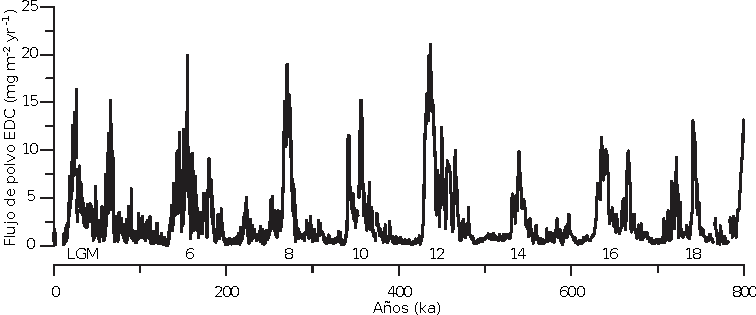
\includegraphics[width=0.9\textwidth]{lambert2008dust.pdf}
 \caption[Polvo en los últimos 800000 años]{Flujo de polvo, obtenido a partir del registro de \textit{EPICA Dome C} (EDC) de los últimos 800000 años. Imagen obtenida y modifica de \cite{lambert2008dust}.}
  \label{fig:dust}
\end{figure}

\cite{martin1990glacial} postula que el polvo mineral tiene un importante rol como fuente de micronutrientes para ciclos biogeoquímicos de la bomba biológica. 

\subsection{Polvo mineral}

\begin{figure}[H]
\centering
 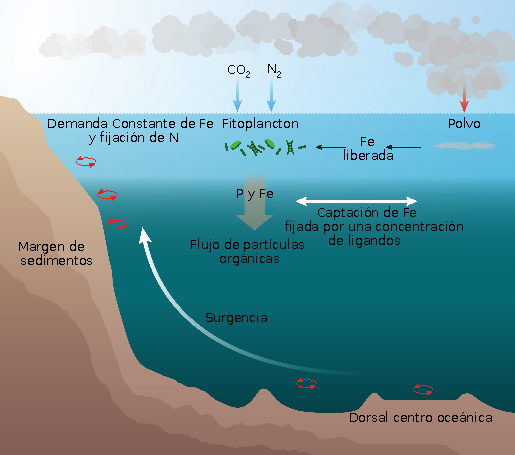
\includegraphics[width=0.75\textwidth]{dustt.pdf}
 \caption[Ciclo del hierro oceánico]{Esquema de la captación y funcionamiento del hierro en los océanos. Modificado de \citep{tagliabue2017integral}.}
  \label{fig:dust0}
\end{figure}

El polvo tiene un importante papel en la dinámica 
del clima, en el balance de energía, la microfísica de las nubes y en la química atmosférica \citep{tegen1994modeling,ridgwell2002dust,mahowald2011aerosol}. 

La erosión eólica en las regiones áridas y semiáridas, son las principales fuentes de flujos de polvo atmosférico (ver figura \ref{fig:dust4}). Esta erosión es una función directa de la velocidad del viento, siempre  y cuando se alcance un umbral que es definido como el límite sobre el cual las partículas comienzan a moverse por procesos de saltación. \cite{iversen1982saltation}, dicen que este umbral existe debido al peso de las partículas del suelo, es decir, que aumenta con el tamaño de grano y la fuerza de cohesión entre ellas que las mantienen sujetas a la superficie. No obstante, también la existencia de elementos no erosionables como la vegetación o rocas aumenta el umbral protegiendo el suelo y consumiendo parte del impulso del viento \citep{marticorena1997factors,tegen1994modeling} así también, la presencia de agua en el suelo aumenta la cohesión de las partículas producto del aumento de las fuerzas capilares entre ellas \citep{bopp2003dust} lo que sumado a la rugosidad, actúa absorbiendo una fracción de la intensidad eólica. De esta manera, la cizalle del viento, junto con el gradiente vertical de velocidad del viento se relacionan de la siguiente manera,

\begin{equation} \label{eq:marco1.5}
\begin{split}
\tau = \mu {\frac{\partial U}{\partial z}}
\end{split}
\end{equation}

Donde $U$ es la velocidad del viento, $z$ es la altura y $\mu$ es la viscosidad dinámica del aire. 

Una ves superado el umbral, los mecanismo que llevan a cabo este levantamiento de material, son: 1) arrastre aerodinámico que requiere de grandes velocidades de viento, 2) saltación, partículas que son lanzadas desde la superficie dibujando una trayectoria balística para impactar la superficie (tienen tamaños que van desde los 70 a 1000 $\mu$m) y 3) degradación de los granos producidos a partir del choque de partículas en la saltación (figura \ref{fig:dust2}). \newpage

\begin{figure}[H]
\centering
 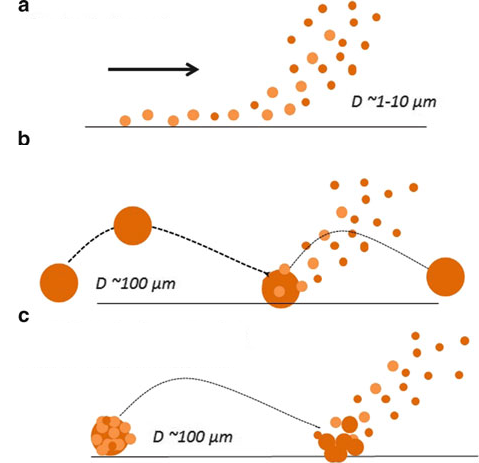
\includegraphics[width=0.5\textwidth]{dust2_pag97book.pdf}
 \caption[Mecanismos de emisión de polvo]{Mecanismos para la emisión de polvo, a) emisión aerodinámica, b) saltación por choque y c) degradación de fragmentos de agregados }
  \label{fig:dust2}
\end{figure}


De este movimiento de partículas sólo una fracción del orden 10$^{-6}$ se convertirá en un flujo vertical (polvo suspendido en la atmósfera) \citep{marticorena1997factors}. Finalmente la velocidad terminal dependerá tanto del peso de la partícula, la velocidad del viento, diámetro y densidad de la partícula, así como de las condiciones atmosféricas.

La generación de polvo es altamente variables según las condiciones locales. Así, entre los requisitos está, que la superficie del suelo esté seca y con poca vegetación, además deben haber altas concentraciones de partículas relativamente grandes (decenas a cientos de micr\'ometros de diámetro) para que el viento las pueda tomar y forzarlas a un movimiento. Esto generará rebotes a través de la superficie, que permitirá un desprendimiento de partículas más pequeñas (menos de 10 a 20 $\mu$m de diámetro) que pueden elevarse a la atmósfera, para recorrer grandes distancias como ``carga'' (ver figura \ref{fig:dust3}). Antes de ser depositadas mediante procesos de sedimentación gravitacional, turbulencia o de precipitación. \newpage

\begin{figure}[H]
\centering
 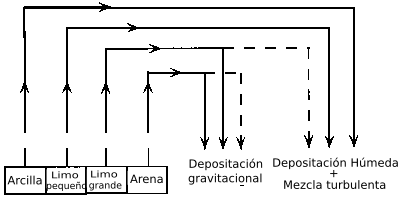
\includegraphics[width=0.65\textwidth]{depositacion.png}
 \caption[Esquema transporte de polvo]{Esquema de transporte de polvo \citep{tegen1994modeling} }
  \label{fig:dust3}
\end{figure}

\cite{prospero2002environmental} usando imágenes del satelitales desde 1978 hasta 1993, tuvo el propósito de identificar la distribución de las principales fuentes de polvo atmosférico, así termina definiendo el ``cinturón global de polvo'' que incluye África el Norte, Península Arabica, Asia Central, China, Australia, América del Norte, Sur África, y la zona sur de Sudamérica (Patagonia). 

\begin{figure}[H]
\centering
 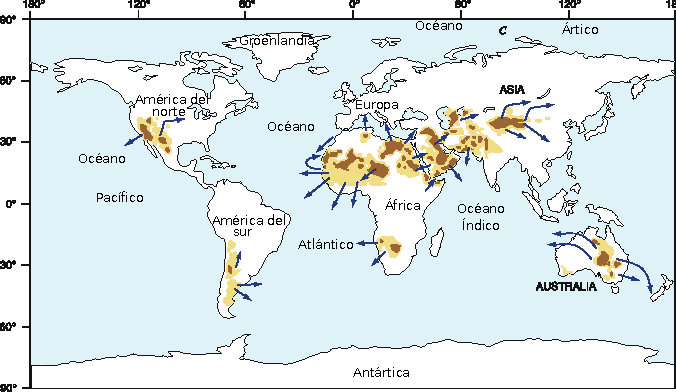
\includegraphics[width=0.9\textwidth]{dust4.pdf}
 \caption[Fuentes de polvo]{Distribución espacial de las fuentes de polvo globales, basada en múltiples imágenes satelitales. Las flechas azules indican las rutas de transporte de polvo \citep{muhs2014identifying}.}
  \label{fig:dust4}
\end{figure} 

Por otro lado, la caracterización mineral del polvo muestra que  el Si es el componente más abundante. Sin embargo, proporciones de Ca, Mg y Fe tienen una diferenciación dependiendo de la fuente. Mientras que elementos como K, Na, Fe, Mn, Ti, P, muestran una distribución mas menos constante \citep{scheuvens2013bulk}. 

Así vemos que el polvo puede llevar consigo nutrientes, los que eventualmente podrían transportarse a grandes distancias. Una de las consecuencias es que puede suministrar fósforo y hierro a ecosistemas terrestres y marinos, lo que modificará los ciclos de productividad de regiones que se encuentran cerca y lejos de las fuentes de polvo \citep{martin1990glacial,anderson2002southern,lambert2015dust,bopp2003dust} (ver figura \ref{fig:dust0}). 

Como se vio en la sección anterior existen zonas oceánicas que están limitadas por hierro (zonas HNLC) o también por fosfato  (giros subtropicales), sin embargo, y a pesar de que el hierro es el cuarto elemento más abundante en las rocas continentales, tiene una muy baja solubilidad (Fe$^{3+}$) \citep{archer2000caused}, que bajo la presencia del oxígeno molecular O$_2$ es rápidamente oxidado de su estado Fe$^{+2}$ (más soluble) en la superficie del océano \citep{martin1990glacial}, así las concentraciones de hierro soluble son cercanas a 1 nmol$^-1$. Del hierro suministrado por el polvo atmosférico, sólo alrededor del $10\%$, está disponible para ser absorbido por el fitoplancton (Fe$^{+2}$). 

En el agua el hierro se encuentra en su forma más oxidada debido a la reacción: 

\begin{equation} \label{eq:marco2.1}
Fe^{3+} + 3OH^{-} \rightleftharpoons Fe(OH)_{3 \textrm{sólido}}
\end{equation}

Por esta razón es que muchos organismo marinos (algas), han desarrollado 
mecanismos para la formación de ligandos \textit{sideroforos}, moléculas que disuelve el ion hierro Fe$^{3+}$ a complejos Fe$^{2+}$ \citep{martin1990glacial,tagliabue2017integral}. Estos ligandos normalmente están unidos a la membrana celular y presentar una gran afinidad por metales traza que transportan. Para el caso del hierro, existen dos tipos de ligandos transportadores, activos los que son producidos por bacterias marinas heterótrofas, hongos y fitoplancton dinoflagelado. Se desarrollan bajo condiciones de limitación del crecimiento, emitiéndose al medio acuático donde reaccionan con el hierro, formando complejos que penetran nuevamente en los organismos, mediante un transporte activo en las proteínas de membrana.
Debido a la alta afinidad de los sideróforos con el hierro Fe$^{3+}$, en condiciones de menor concentración que el hierro se encuentra completamente unidos al metal. 

Por lo tanto, dentro del oc\'eano el hierro esta fusionado org\'anicamente 
y siendo constantemente reutilizado teniendo un tiempo de residencia de unos meses a años \citep{boyd2010biogeochemical}.

La limitaci\'on de hierro en aguas superficiales refleja concentraciones que son inadecuadas para la formaci\'on de fitoplancton debido a que la regeneraci\'on de \'este es m\'as lenta que el 
hundimiento de hierro contenido en materia org\'anica. As\'i para el mantenimiento de la producci\'on primaria del oc\'eano abierto se requiere un aporte mayor que el dado por el afloramiento, el cual generalmente es atmosf\'erico.

As\'i la absorci\'on de hierro por algunos fitoplancton hacen que este influya en la comunidad de algas, y por tanto, en la productividad en general. Cabe destacar que el fitoplancton de mar abierto 
por lo general requiere de menos hierro que las especies costeras, las que se han desarrollado en un ambiente rico en hierro. As\'i se ha logrado un requerimiento menor de hierro reduciendo el tama\~no
de las c\'elulas y minimizando el n\'umero de enzimas que contienen hierro \citep{palenik2003genome}. Sin el estr\'es de hierro veremos presencia de fitoplancton con c\'elulas m\'as grandes. 

Aparte de la limitaci\'on directa de la
producci\'on primaria en las zonas HNLC el hierro puede limitar la fijaci\'on de nitr\'ogeno de las especies fotosint\'eticas. 

En las regiones HNLC los cambios en el suministro de hierro afectar\'an directamente la producci\'on primaria y la composici\'on de las especies, mientras que en las regiones oligotr\'oficas
subtropicales/tropicales el impacto ser\'a principalmente a trav\'es de cambios en la fijaci\'on de nitr\'ogeno \citep{jickells2005global}. 

Por otro lado, dado que la solubilidad del hierro es baja se estima que hay grandes concentraciones de part\'iculas de hierro en el onc\'eano profundo, de esta manera si parte de este polvo se disuelve en profundidad aumentar\'an las concentraciones abisales de hierro disuelto, y a largo plazo la productividad en las regiones de surgencia como 
los oc\'eanos del sur \citep{parekh2005decoupling}. 

\section{Última deglaciación}

El Pleistoceno se ha caracterizado por ciclos glaciares/interglaciares que han tenido terminaciones abruptas, donde llegan a un máximo interglacial que generalmente ocurre al comienzo del interglacial, luego se produce un descenso de las temperaturas para comenzar una glaciación, posteriormente las temperaturas descienden hacia un máximo glacial. Se sabe que estos periodos han estado sujetos a variaciones relacionadas con parámetros orbitales de la Tierra denominados ``ciclos de Milanckovitch'', que tienen periodos de 100, 41 y 23 mil años, donde particularmente los últimos 800 mil años han tenido una periodicidad de 100 ka. 

\begin{figure}[H]
\centering
 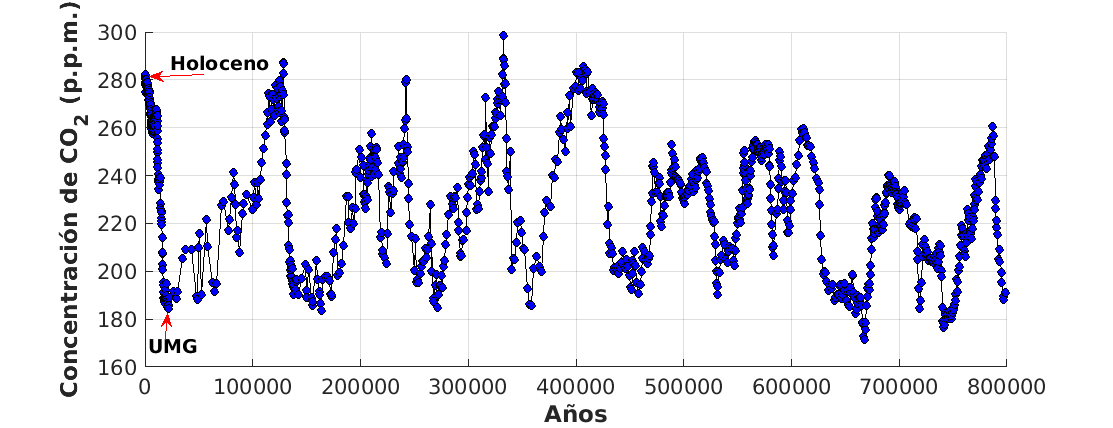
\includegraphics[width=1\textwidth]{CO2glob.png}
 \caption[Registro de CO$_2$, últimos 800 mil años]{Registro de CO$_2$ de los últimos 800000 mil años. Datos obtenidos de \citep{luthi2008high}. }
  \label{fig:CO2}
\end{figure}

La última deglaciación corresponde a la transición entre el periodo de máximo estadial del último ciclo del cuaternario (ocurrido aproximadamente hace 21000 años a.p.) \citep{clark2009last}, conocido como el Último Máximo Glacial (UMG), y el comienzo del Holoceno (\string~ 12000 años  a.p.) \citep{sigman2000glacial,barker2009interhemispheric}.


\subsection{\'Ultimo m\'aximo glacial}
 
 El UMG es el periodo más frío dentro del último periodo glacial correspondiendo al rango de tiempo desde 26.5 ka a 21 ka \citep{clark2009last}. Gracias a diversos paleoproxies, es sabido que durante este periodo 
las concentraciones de pCO$_2$ fueron cercanas a las 180 partes por millón por volumen (p.p.m.v) \citep{luthi2008high}, habían bajas temperaturas, el nivel del mar era 120 m. más bajo que el nivel
 actual \citep{fairbanks198917,denton2010last,lambeck2014sea} debido a una gran expansión de los casquetes de hielo polar como es el caso de Laurentide en el Hemisferio Norte que fue creciendo desde el comienzo de la última glaciación hasta alcanzar su máxima extensión en el UMG \citep{fairbanks198917}, y el océano global era 3\% más salado que en la actualidad \citep{sigman2000glacial,bopp2003dust}. Además diversos modelos y registros paleoclimáticos han mostrado que habían mayores flujos de polvo, debido a posibles aumentos del área de las fuentes, y/o por intensificación de los vientos o disminución del ciclo hidrológico \citep{mahowald1999dust,lambert2008dust,maher2010global}. 

\begin{figure}[H]
\centering
 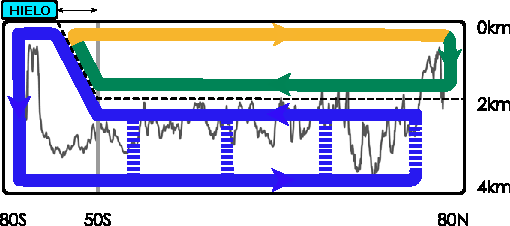
\includegraphics[width=0.6\textwidth]{LGMWater.pdf}
 \caption[Circulación de volcamieno en el LGM]{\textit{Circulación de volcamieno en el LGM.} La linea azul es el agua proveniente de la Antártica que llena las profundidades abisales e intermedias del océano, mientras la barra verde es el agua del Atlántico Norte que llegaba a profundidades intermedias, y la linea amarilla es la Agua Intermedia Antártica. Imagen obtenida y modifica de \citep{ferrari2014antarctic}.  } 
\label{fig:aguaCO2}
\end{figure}

 Por otro lado, la circulación oceánica durante este periodo se cree fue más estratificada (ver figura \ref{fig:aguaCO2}) \citep{sigman2000glacial,lynch2007atlantic,tagliabue2009quantifying,ferrari2014antarctic}. Una de las teorías de esta mayor estratificación es debido al carácter estacional de la formación de capa de hielo del Hemisferio Norte (en invierno se crea volumen de hielo y en verano el agua se refresca por derretimiento). Esto según \cite{ferrari2014antarctic}, habría producido durante el UMG un resfrescamiento del agua en el Atlántico Norte, lo que produciría que las aguas superficiales provenientes de las zonas ecuatoriales no lograran niveles de densidad suficiente para producir un volcamiento adecuado, por esta razón las formación de aguas del Atlántico Norte no habrían superado profundidades mayores a 2 km. Así se dice que durante el UMG el volumen oceánico fue llenado por aguas de origen Antártico. No se habría producido la \textit{Agua Profunda Circumpolar} (CDW) por lo tanto los regímenes no habrían mantenido contacto producto de mezcla vertical. Otro teoría es propuesta por \cite{toggweiler2006midlatitude}, que se refiere a un debilitamiento de la CDW como resultado de un movimiento hacia el ecuador de los \textit{vientos del oeste} durante periodos glaciares, lo que conduciría a menor divergencia de agua superficial, por lo tanto, a menor surgencia de agua profunda. 

 Además, el volumen de hielo marino se habría expandido hasta el \textit{Frente Polar Antártico} durante invierno, y a niveles cercanos a los actuales durante el verano \citep{bopp2003dust}. Esto tienen particular importancia en los Océanos del Sur dado que es en esta zona donde se refrescan las aguas densas, con mucho contenido de CO$_2$ (producto de la respiración oceánica) y nutrientes provenientes del océano Atlántico, Indico y Pacifico (ver sección Bomba Biológica). Por esta razón, un aumento de la cobertura de hielo de la zona Antártica, habría generado un bloqueo de gran parte de la surgencia de agua profunda, afectando de esta manera tanto la liberación de CO$_2$ como, los ciclos biogeoquímicos del océanos. 

\subsection{Terminación I}

Como se mencionó y se puede apreciar en la figura \ref{fig:CO2}, todos los ciclos glaciares han finalizado por un abrupto cambio desde un estado de máxima glaciación a un estado de rápidos incrementos de temperatura. La última transición Glaciar-Interglacial no es la excepción a esta regla. 

La terminación I, comenzó hace aproximadamente 21000 años atrás en el Hemisferio Norte, y hace aproximadamente 18000 años atrás en el hemisferio Sur \citep{denton2010last,clark2009last,lynch2007atlantic}.  Lo anterior debido al comportamiento dipolar entre los hemisferios, finalizando aproximadamente hace 12000 años atrás. 

\cite{denton2010last}, propuso una serie de factores que a su juicio podrían haber gatillo el comienzo de este periodo de transición. Todo comienza con un aumento de la insolación de verano en el Hemisferio Norte (H.N), sin embargo, esto es insuficiente para explicar la rápida y gran variación. Así lo anterior, en conjunto con una gran extención de la cubierta de hielo del Hemisferio Norte, habría generado una presión isostática del hielo que no fue posible mantener provocando grandes eyecciones de flujos de hielo y agua dulce producto del derretimiento y la ablación, a zonas de hundimiento de agua en el Atlántico Norte, afectando la circulación de volcamiento \citep{ferrari2014antarctic}. Producto de cambios de temperaturas del agua superficial, la zona de \textit{interconvergencia intertropical}
fue desplazada hacia el sur. Mientras tanto, el Hemisferio Sur que se mantenía en sus condiciones glaciales, en la zona Antártica se comenzaron a derretir los casquetes de hielo producto de un desplazamiento de los vientos del oeste hacia los polos, incrementando la surgencia en la \textit{Corriente Circumpolar Antártica} (ACC) lo que produjo una liberación de CO$_2$, que habría amplificado el efecto de incremento de temperaturas medias. 

Sin embargo, este periodo no estuvo exento de variaciones climáticas tanto en el H.N. como en el H.S. además de la evidencia que se ha mostrado acerca de la asincronía interhemisférica lo que se ha denominado el ``balancín dipolar''. Así, luego de dar comienzo a la Terminación I en el H.N. registros han mostrado un enfriamiento en el Atlántico Norte, conocido como \textit{Heinrich estadial 1} (HS1), mientras en el mismo lapsus de tiempo en el Hemisferio Sur significó el comienzo de la transición. El mismo efecto es visto por la llamada \textit{Reversión fría Antártica} (ACR) en el H.S. lo que en el H.N. se ve reflejado como un periodo cálido denominado intervalo \textit{Bølling–Allerød} ($\sim 14.7$ mi años) \citep{renssen2001two}, luego en el Hemisferio Norte hay evidencia de un nuevo periodo frió conocido como \textit{Younger Dryas} ($\sim 12.8–11.5$ mil años) lo que implicó la completa deglaciación del H.S. \citep{denton2010last,barker2009interhemispheric}.

\subsection{Holoceno}

Así se llegaría entonces al fin del periodo Cuaternario y comienzo del Holoceno, con una concentración atmosférica de CO$_2$ en torno a las 280 p.p.m. \citep{sigman2000glacial}. Pero que desde el periodo preindustrial, ha ido en aumento.

 Esta época al igual que la Terminación I se ha caracteriza por una marcada inestabilidad. Con una fuerte relación con la irradiansa solar, generando ``ciclos'' con una periodicidad promedio de 1500 años en el Hemisferio Norte \citep{bond2001persistent}. Afectando la posición de la \textit{Zona de Interconvergencia Tropical} (ITCZ) \citep{haug2001southward}, y la posición e intensidad de los vientos del oeste \citep{moreno2010covariability,lamy2010holocene}. Así en periodos con una baja irradiansa solar, en el Hemisferio Norte hay registros de grandes apariciones de hielo a la deriva, enfriando el océano superficial y la temperatura atmosférica de Groenlandia, lo que se traduce en una reducción de la precipitación en latitudes medias \citep{bond2001persistent}. 

 Respecto de la fuentes y niveles de polvo atmosférico, éstos tienen una notable disminución, como tanto los registros como los modelos muestran (ver sección 4.1) \citep{mahowald1999dust,kohfeld2001dirtmap} debido presumiblemente, a la disminución de la intensidad de los vientos.

\section{Modelos}

\begin{figure}[H]
\centering
 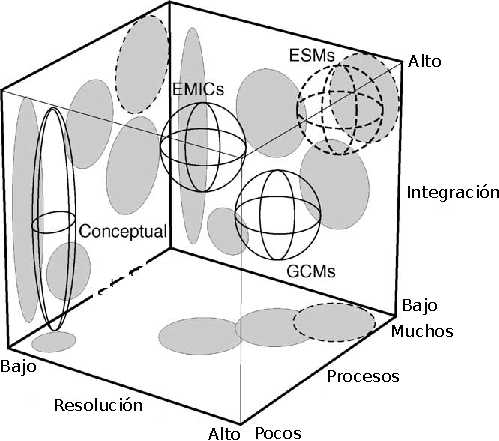
\includegraphics[width=0.5\textwidth]{modelos2.pdf}
 \caption[Tipos de modelos]{Grado de complejización de los modelos, en función de su nivel de resolución y procesos que incluyen. El modelo en línea punteada corresponde a los \textit{Modelos de Sistema Tierra}. Figura adaptada de \citep{bartlein2003modeling}. }
  \label{fig:modelos}
\end{figure}

El sistema climático se considera formado por componentes que tienen características bioticas y abioticas, tal como, la geósfera que incluye la atmósfera, hidrósfera (principalmente ríos y océanos), la criósfera (hielo marino, permafrost, hielo interior y cubierta de nieve), la pedósfera (suelo) y la litosfera (corteza terrestre y manto superior de la Tierra), sistemas abiertos que en conjunto son conocidos como el sistema climático físico, que interaccionan con la componente biosférica. 

Con el desarrollo de la ciencia computacional, el progreso de la termodinámica en los años 90s y el creciente interés por entender los procesos que gobiernan la variabilidad climática es que se sentaron las primeras bases de los principios físicos que gobiernan el flujo atmosférico \citep{lynch2008origins}.  Con ello se dio paso desde los modelos conceptuales a los modelos más complejos que integraban las atmósfera y el océano (ESM, \textit{Modelos del Sistema Tierra}) \citep{flato:hal-01644494}. 

Los tipos de modelos se diferencias en su grado de complejidad, es decir, el grado de componentes que posee y utiliza para reproducir el sistema Tierra \citep{weber2010utility}.

 Los modelos conceptuales están basados en conceptos del funcionamiento del sistema Tierra, diseñados para ser computacionalmente eficientes. Entre estos destacan los \textit{Modelos de Balance Energéticos} (EBMs, por sus siglas en inglés) y los modelos de caja. Los primeros, resuelven el balance de calor radiativo de la atmósfera en términos de la temperatura superficial del aire. Existen en una y dos dimensiones. Otros, son los modelos de caja, modelos simples con baja resolución espacial cuyas cajas son representaciones de relaciones biogeoquímicas, que sacrifican el grado de realismo físico pero dan una exploración de los parámetros espaciales en cuestión.

  Por otro lado, se encuentran los modelos más complejos \textit{Modelos de Circulación General} (GCM, por sus siglas en ingles), pero menos integrados que se enfocan en la dinámica atmosférica y del océano. Son modelos que resuelven la ecuación fundamental de movimiento, junto con la evolución de la temperatura y humedad de la atmósfera o la temperatura y salinidad de los océanos. Contienen una baja cantidad de componentes que son directamente acopladas. Estos modelos son más realistas, pero poseen un alto costo computacional, por lo que son usados mayormente para experimentos multidecadales, aunque tambi\'en para an\'alisis del tiempo sin\'optico un subconjunto conocido como \textit{Modelos Climáticos Regionales.} Los \textit{Modelos de Sistema Tierra de Complejidad Intermedia} (EMICs, por su sigla en inglés), es un tipo de modelo acoplado (lo que permite escoger los m\'odulos que se desean simular en funci\'on de la pregunta que se plantea), que se encuentra en el medio de los dos comentados anteriormente (ver figura \ref{fig:modelos}), estos describen el sistema climático con menos detalle espacial y temporal que los GCMs, con mayor simplicidad de sus componentes físicas, pero incluyen más procesos integrados de forma parametrizada, lo que permite una mayor interacción de los módulos al representar procesos y un bajo costo computacional (ver tabla \ref{tabla:modelos}), a la vez que tambi\'en pueden integran balances biogeoquímicos \citep{claussen2002earth,flato2011earth}. Además se diferencia de los modelos conceptuales dado que sus grados de libertad exceden (por mucho) las parametrizaciones que posee \citep{weber2010utility}. Los EMICs, fueron diseñados para reproducir escalas de tiempo que están entre 10$^2$ y 10$^5$ años. Permiten hacer simulaciones de sensibilidad. Finalmente, los \textit{Modelos de Sistema Tierra} (ESMs, por su sigla en ingl\'es), son modelos acoplados interactivamente que integran tanto las din\'amicas de la circulaci\'on vistas en los GCMs como las caracter\'isticas que son manejadas por los EMICs, siendo un modelo altamente integrado pero que se caracterizan adem\'as, por una alta resoluci\'on espacial aunque computacionalmente limitados \citep{bartlein2003modeling}. 


\begin{table}[H] 
\centering
\resizebox{12cm}{!} {%
\begin{tabular}{|cc|}
\hline \hline
\multicolumn{2}{c}{\bf Parametrización} \\
%\cline{2}
\hline \hline
Componentes & Características  \\
\hline \hline
\multirow{3}{*}{Atmósfera}  & Convección y microfísica de nubes  \\ \cline{2-2}
& Aerosol e interacciones \\ \cline{2-2}
& Capa límite \\ \cline{2-2}
& Radiación \\ \hline
Océano& Difusión y advección de remolinos \\ \hline
\multirow{2}{*}{Tierra} & Vegetación/Tipo de suelo \\ \cline{2-2}
& Humedad \\ \cline{2-2}
& Nieve o agua subterránea \\ \hline
Cubierta de hielo & Propiedades dinámicas y termodinámicas \\ \hline
\multirow{4}{*}{ * Ciclo de carbono} & Procesos químicos y biogeoquímicos \\ \cline{2-2}
& Captación de CO$_2$ \\ \cline{2-2}
& Especies de plancton y fitoplancton \\ \cline{2-2}
& Inclusión de carbonato de calcio (CaCO$_3$) \\ \cline{2-2}
& Partículas de aerosol\\ \hline
\multirow{2}{*}{ * Partículas de aerosol} & Ciclo de azufre \\\cline{2-2}
& Efecto directo e indirecto del aerosol de sulfato \\ \cline{2-2}
& Polvo en aerosol \\ \hline 
\multirow{1}{*}{ * Ciclo de metano y permafrost} & Química atmosférica del CH$_4$ \\ \cline{2-2}
& Emisiones de CH$_4$ en humedales \\ \hline
\multirow{2}{*}{ \makecell{* Dinámica global de la vegetación\\ e incendios forestales}} & \makecell{hidrología del suelo \\ (superficial y subsuperficial)} \\ \cline{2-2}
& descarga de agua en ríos \\ \cline{2-2}
& Intercambio de agua con la atmósfera \\ \cline{2-2}
& Fuentes ecológicas \\ \cline{2-2}
&  \makecell{Interacción del ciclo del carbono \\ inclusión de Gases trasas CH$_4$, N$_2$O y NO$_X$} \\ \hline
* Uso y cambio de suelo & \makecell{Tratamientos de cultivos \\ e interacción con el paisaje y zonas urbanas}\\ \hline
\multirow{2}{*}{\makecell{ * Interacciones químicas del clima y \\ acoplamiento estratosférico - troposférico}} & Circulación troposférica \\ \cline{2-2}
& Dinámica estratosférica \\ \cline{2-2}
& Interacción dinámica estratosférica - troposférica \\ \hline
* Capas de hielo en la tierra & \makecell{Tasa de agua derretida provenientes \\ de la Antártica y Groenlandia} \\ \hline
\multirow{3}{*}{\makecell{* Características adicionales \\ acoplamiento Océano-Atmósfera}} & Corrientes oceánicas superficiales \\ \cline{2-2}
& Radiación solar que penetra en el océano \\ \cline{2-2}
& Captura de radiación por la clorofila \\ \cline{2-2}
& Distribución de clorofila \\ \hline \hline
\end{tabular}%
}
\caption[Componentes de modelos]{Componentes de los modelos GCMs y EMICs. Los marcados con asterisco son los que sólo se incluyen en los modelos EMICs y ESM. } 
\label{tabla:modelos}
\end{table} 
